\section{Introduction}

\begin{frame}[fragile, allowframebreaks]{Introduction}

\begin{block}{Acknowledgement}
A special thanks to {\bf CeSeNA Security} group and \emph{Marco Ramilli} our ``old'' mentor...
\end{block}

\begin{block}{Where to find us}
\begin{itemize}
\item Website: {\small \url{http://cesena.ing2.unibo.it/}}
\item GitHub: {\small \url{https://github.com/cesena}}
\item We have also an IRC channel on freenode and a Google Group!
\end{itemize}
\begin{flushright}

\includegraphics[height=1cm]{imgs/CeSeNA.png}
\end{flushright}
\end{block}

\framebreak

\begin{block}{Before smashing things}
We need to say some words about security in general :) !
\end{block}

\framebreak

\begin{block}{Security facts in modern era}
\begin{itemize}
\item Each security breach costs over 500k to Corporates\\
{\small \url{http://goo.gl/RAUgOg}}
\item Cyber-Security market is growing (\emph{63 billion in 2011, 120 billions in 2017})\\ {\small \url{http://goo.gl/Zq8Efj}}
\item Zero-Day exploit black markets, and Bug-Bounty (\emph{yes Microsoft is doing it too})
\end{itemize}
\end{block}

\framebreak

\begin{block}{Is someone still using C}
Lot of C/C++ out there.. {\small \url{http://langpop.com/}  \url{http://www.tiobe.com/} }
\end{block}

\begin{block}{Buffer OverFlows are old stuff}
\begin{center}
\begin{tabular}{l|c}
\hline
Who  & \emph{Adobe Reader and Acrobat} \\
\hline
What & \emph{stack-based buffer overflow} \\
\hline
When & \emph{ \bf \color{red} 2014 } \\
\hline
\end{tabular}
\end{center}
\hfill \emph{Check CVE-2014-8460}
\end{block}

\end{frame}

\subsection{Smashing the stack}

\begin{frame}[fragile, allowframebreaks]{Smash the stack}
\begin{block}{\emph{Smash The Stack} [C programming] n.}
\begin{itemize}
\item On many C implementations it is possible to {\bf corrupt the execution stack} by \underline{writing past the end of an array} declared auto in a routine.
\item Code that does this is said to smash the stack, and \emph{can cause return from the routine to jump to a random address}.
\end{itemize}
\begin{center}
\bf This can produce some of the most insidious data-dependent bugs known to mankind.
\end{center}
\end{block}
\end{frame}

%%%%%%%%%%%%%%%%%%%%%%%%%%%%%%%%%%%%%%%%%%%%%%%%%%%%%%%%%%%%%%%%%%%%%%%%
\subsection{Stack Frame}
\begin{frame}[fragile, allowframebreaks]{Stack Frame}

\begin{columns}[T]
	\begin{column}{.6\textwidth}
	\begin{itemize}
\item Logical \emph{frames} pushed during function calls and popped when returning.
\item {\bf stack frame} contains the \underline{function params}, its \underline{local variables}, and the necessary \underline{data for recovering previous frame}.
\item So it also contains the value of the {\bf instruction pointer} at the time of the function call.
\item Stack grows down (towards lower memory addresses)
\item The \underline{stack pointer} points to the last used address on the stack frame.
\item The \underline{base pointer} points to the bottom of the stack frame.
\end{itemize}
	\end{column}
	\begin{column}{.3\textwidth}
	\tiny\begin{verbatim}
|                              0xffff
|           <--- Previous
|                Stack Frame
|===FRAME=BEGIN===
| PARN
|  ..
| PAR2      <--- Parameters
| PAR1
|-----------
| OLD_EIP
| OLD_EBP   <--- EBP points here
|-----------
| Var 1
|  ..
| Var N     <--- ESP points here
|====FRAME=END====
|
|
|                             0x0000
	\end{verbatim}


	\end{column}
\end{columns}



\framebreak

\begin{block}{Stack in x86-x86\_64}
Stack grows in opposite direction w.r.t. memory addresses.\\
Also two registers are dedicated for stack management:
\begin{description}
\item[EBP/RBP], points to the {\bf base} of the stack-frame (\emph{higher address})
\item[EIP/RIP], points to the {\bf top} of the stack-frame (\emph{lower address})
\end{description}
\end{block}

\begin{block}{Who setup the stack frame?}
Calling convention:
\begin{itemize}
\item Parameters are pushed by caller.
\item \emph{EIP} is pushed via \emph{CALL instruction}.
\item \emph{EBP} and local vars are pushed by called function.
\end{itemize}
\hfill \tiny Valid for x86\\
\hfill x86-64 uses different convention (FAST-CALL)
\end{block}

\framebreak

\begin{block}{Call Prologue and Epilogue}
\begin{columns}[c]
    \column{.4\textwidth}
    \acode
    \tiny
\begin{lstlisting}
call fun   ;push EIP
\end{lstlisting}
    \column{.4\textwidth}
     \acode
     \tiny
\begin{lstlisting}
  fun:
  push EBP ; prologue
  mov EBP, ESP
  sub ESP,<paramspace>
  ...
  ; epilogue
  mov ESP, EBP
  pop EBP ;restore EBP
  ret     ;pop EIP
\end{lstlisting}
\end{columns}
\end{block}

\framebreak

\begin{block}{Stack Frame: Recap}
Logical \underline{stack frames} that are \emph{pushed in the .stack segment} on function call, popped when returning.\\
A stack frame contains:
\begin{itemize}
\item Parameters (depends on calling convention, not true for linux64)
\item {\bf Data for previous frame recovering, also old Instruction Pointer value}.
\item Local variables
\end{itemize}
\end{block}

\framebreak

\begin{figure}[tb]
  \centering
  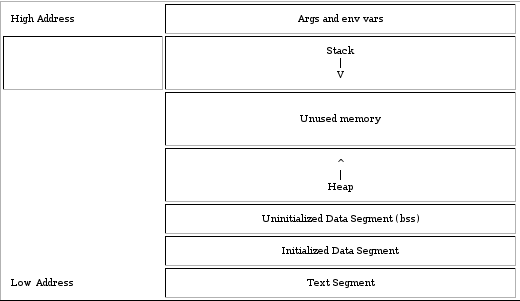
\includegraphics[width=0.8\linewidth,keepaspectratio]{imgs/VMspace.png}
  \caption{VM space}
  \label{fig:vmspace}
\end{figure}
\end{frame}
